\section{Preferences}
\label{sec:Preferences}
AstroJournal allows users to customise a few parameters via graphical user interface (Edit $\rightarrow$ Preferences).\\
If you are acquainted with Latex, you can also change the generated document headers and footers by editing the files in the folder latex\_header\_footer. No customisation is required for a normal use of AstroJournal.

\begin{center}
\begin{figure}
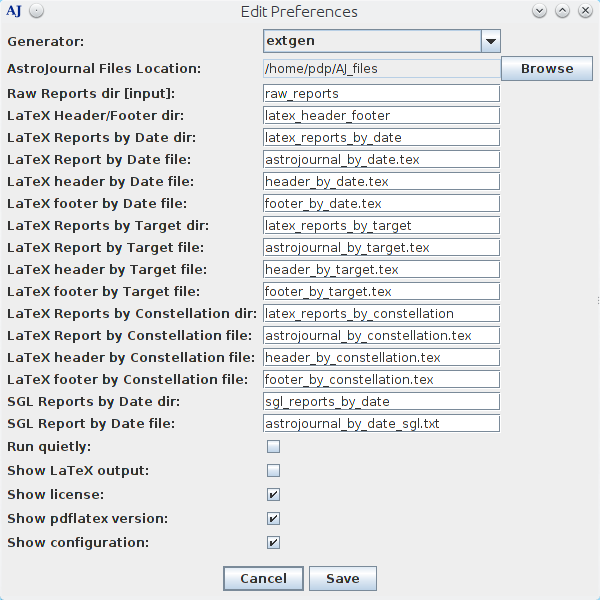
\includegraphics[width=1.0\textwidth]{images/preferences}\par\vspace{1cm}
\caption[AstroJournal customisation]{By default AstroJournal exports every fields provided in the csv or tsv files. However, it is also possible to export more compact reports by selecting a different generator. The ``Location'' field determines the folder where the raw reports (csv or tsv files) are stored. Users can also customised the name of output files and directories. If desired, the output on the main AstroJournal window can also be personalised. Two useful test features are ``Show pdflatex version'' and ``Show LaTeX output''. When enabled, the former will show the output of the command pdflatex -version. This can be useful for testing the correct installation of pdflatex. The latter will show the complete output produced by pdflatex when exporting from LaTeX to PDF format.}
\end{figure}
\end{center}
